\documentclass{standalone}
%
\usepackage{tikz}
\usepackage{xcolor}
%
\definecolor{glass}{HTML}{BCFBF7}
\definecolor{water}{HTML}{2E889A}
%
\title{Ghiaccio nel bicchiere}
\begin{document}
	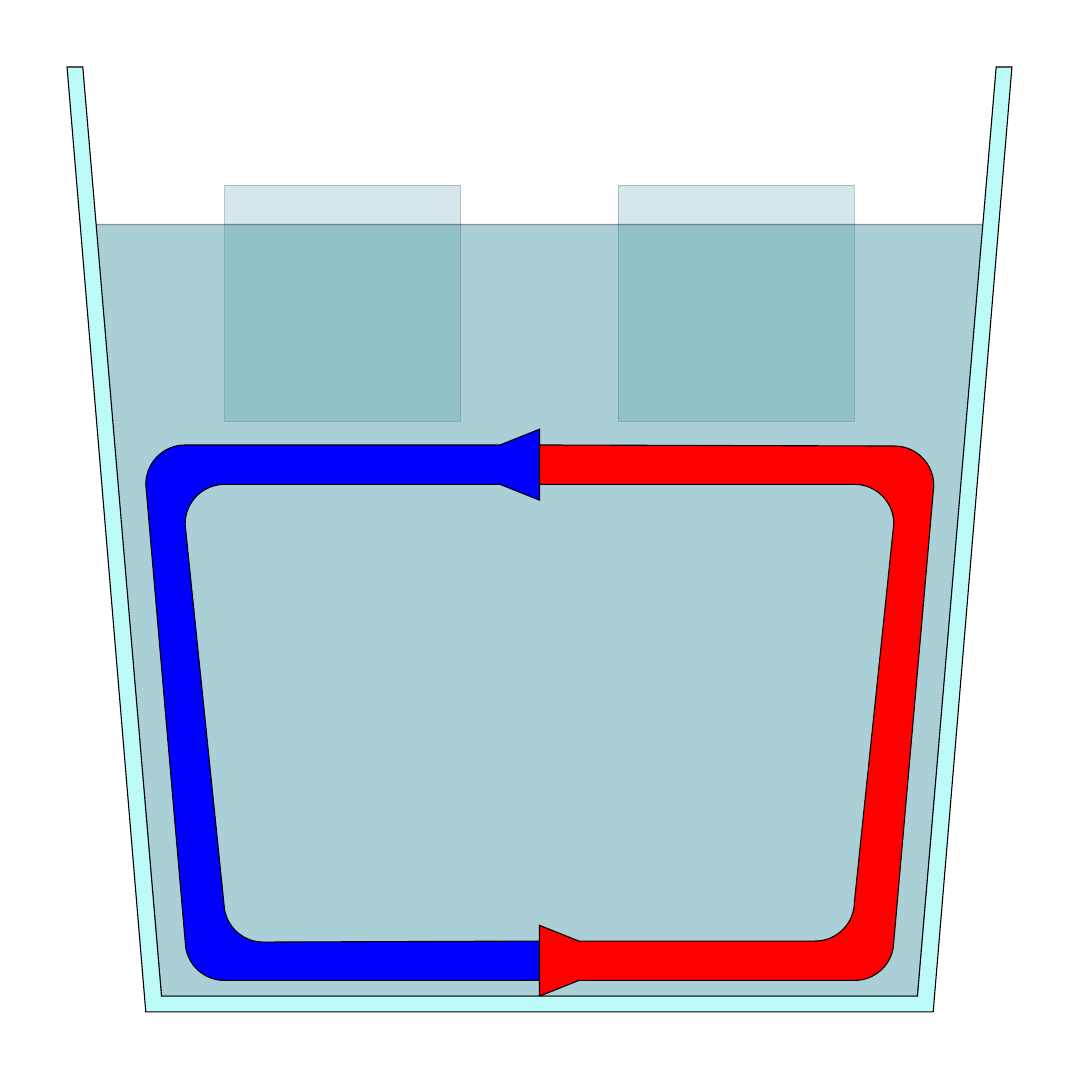
\begin{tikzpicture}
		\fill [white] (-6.5,12.5) rectangle (6.5,-0.5);
		\draw [fill=water,opacity=0.2] (-4,10.5) -- (-1,10.5) -- (-1,7.5) -- (-4,7.5) -- (-4,10.5);
		\draw [fill=water,opacity=0.2] (4,10.5) -- (1,10.5) -- (1,7.5) -- (4,7.5) -- (4,10.5);
		\draw [fill=water,opacity=0.4] (-5.64,10) -- (5.64,10) -- (4.8,0.2) -- (-4.8,0.2) -- (-5.64,10);
		%
		\draw [fill=blue] (0,6.7) -- (0,6.5) -- (-0.5,6.7) -- (-4,6.7) arc (90:190:0.5) -- (-4,1.3) arc (190:270:0.5) -- (0,0.9) -- (0,0.4) -- (-4,0.4) arc (270:190:0.5) -- (-5,6.7) arc (180:90:0.5) -- (-0.5,7.2) -- (0,7.4) -- (0,6.7);
		\draw [fill=red] (0,0.2) -- (0.5,0.4) -- (4,0.4) arc (270:350:0.5) -- (5,6.6) arc (-370:-270:0.5) -- (0,7.2) -- (0,6.7) -- (4,6.7) arc (-270:-360:0.5) -- (4,1.4) arc (360:270:0.5) -- (0.5,0.9) -- (0,1.1) -- (0,0.2);
		\draw [fill=glass] (5,0) -- (6,12) -- (5.8,12) -- (4.8,0.2) -- (-4.8,0.2) -- (-5.8,12) -- (-6,12) -- (-5,0) -- (5,0);
	\end{tikzpicture}
%
\end{document}
